\chapter{Background and Literature}
\label{ch:background}

This chapter introduces technical concepts and background used in the conceptualized solution of the thesis. It also explains the state of the art of the different technologies used in the thesis and the current state of research in sound source localization and distance estimation.

\section{Sound Propagation}

Sound propagation is the physical process by which sound waves propagate in a given environment. The strength of the sound wave depends on various factors, including the frequency, environment, and distance from the sound source. These factors make an accurate identification and localization of a sound source difficult; thus, a more accurate and robust sound source localization system is needed.

\subsection{Realistic sound propagation in simulations}

\subsection{Microsoft Project Acoustics}

Microsoft Project Acoustics is a sound propagation engine that simulates the propagation of sound waves in a given environment. It is used in various applications, including video games, virtual reality, and augmented reality. It simulates wave effects like obstruction, reverberation, and occlusion in complex 3D scenes without requiring zone markup or raytracing. It works similarly to a raytracing engine but is precomputed and optimized for real-time performance. 

\subsection{Sound Propagation in game-engine}

\section{Sound Source Localization}

Sound Source Localization (SSL) is the process of determining the position of a sound source. It usually uses a microphone array that captures the sound signals from multiple directions. SSL is used in various applications, such as speech recognition, robot navigation, surveillance, and security. In this thesis, SSL is used to estimate the distance and direction of a sound source to detect excessively noisy vehicles.

\subsection{Spectrograms for sound visualization}

Spectrograms are a visual representation of the frequency content of a sound signal. They are often used in sound source localization to identify the direction of a sound source. The spectrogram is a two-dimensional representation of the frequency content of a sound signal (figure \ref*{fig:spectrogram_example}).

\begin{figure}[H]
    \centering
    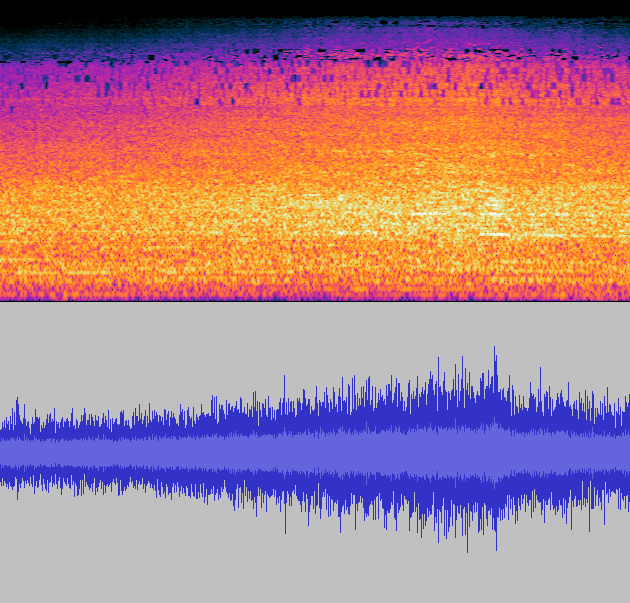
\includegraphics[width=0.5\textwidth]{../Images/spectrogram-example.png}
    \caption{Spectrogram of a sound signal}
    \label{fig:spectrogram_example}
\end{figure}

The x-axis represents time, and the y-axis represents frequency. The intensity of the color at each point in the spectrogram represents the amplitude of the frequency component. A matrix of spectrograms allows the representation of multiple channels, such as the ones recorded by a microphone array. On that matrix, each spectrogram represents the frequency content of a single channel (figure \ref*{fig:2_channel_spectrogram_example}).

\begin{figure}[H]
    \centering
    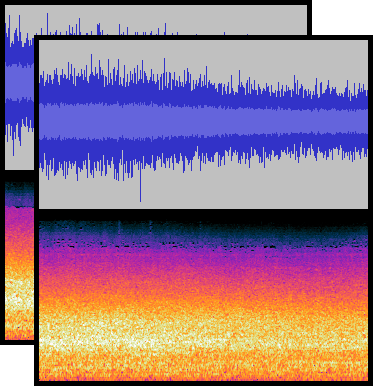
\includegraphics[width=0.4\textwidth]{../Images/2-channel-spectrogram-example.png}
    \caption{Dual channel spectrogram matrix of a sound signal}
    \label{fig:2_channel_spectrogram_example}
\end{figure}

Looking at the frequency content of the sound signal allows us to identify the time delta of a recorded sound by using a multi-channel spectrogram. The bright spot on the spectrogram will indicate a jump in the amplitude and determine the start time of the record of a loud sound. By comparing this time with the other channel, we can find the direction of the sound source by comparing the sound signal's time delta with the other channels' time delta (figure \ref*{fig:spectrogram_offset}).

\begin{figure}[H]
    \centering
    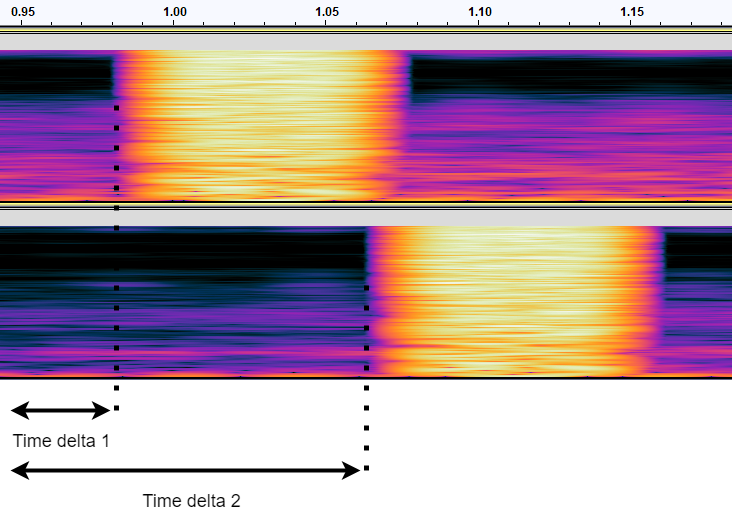
\includegraphics[width=0.5\textwidth]{../Images/time_delta.png}
    \caption{Spectrogram of two sound signals with time their delta}
    \label{fig:spectrogram_offset}
\end{figure}

Since we know the distance between the microphones, we can determine the direction of the sound.

\subsection{Origin of sound using two microphones}

Admitting the following setup (figure \ref*{fig:microphones_setup}), if the time delta 1 is greater than the time delta 2 of the other channels (setup 1), the sound source is closer to microphone 2. If the time delta 1 equals the time delta 2 (setup 3), the sound source is at the same distance to both microphones. If the time delta 2 is greater than the time delta 1 (setup 2), the sound source is closer to the microphone 1. 

\begin{figure}[H]
    \centering
    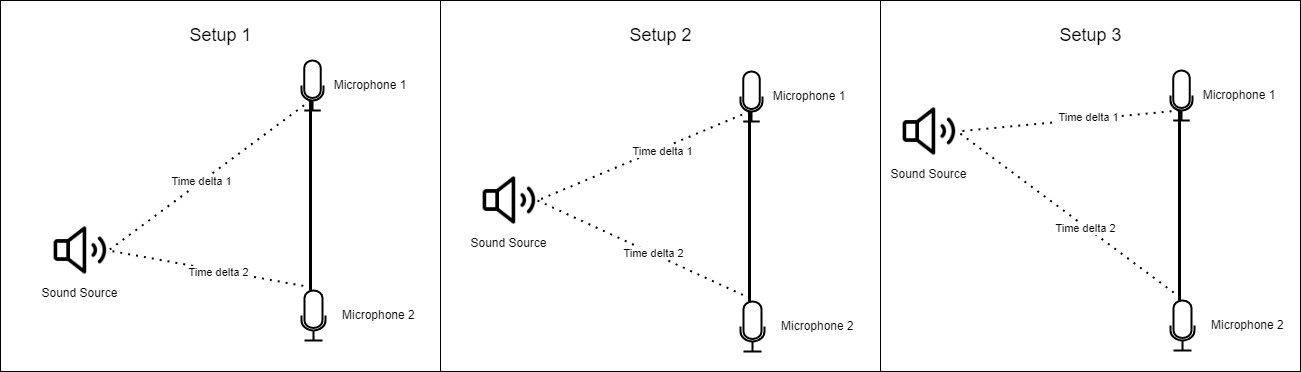
\includegraphics[width=1\textwidth]{../Images/microphones_setups.png}
    \caption{Sound source localization setup}
    \label{fig:microphones_setup}
\end{figure}

This concept can be formalized and is better explained in \cite{Scola2010DirectionOA}. Once the delay between the two microphones is known, the equation allows us to find the direction of the sound source by using trigonometric calculations. As in the figure \ref*{fig:sound-source-from-two-microphones}, considering point $M$ as the sound source and point $A$ and $B$ as microphones, the distance between the two microphones is $d$ and the time delta between the two microphones is $\Delta t$, the angle $\alpha$ can be calculated.

\begin{figure}[H]
    \centering
    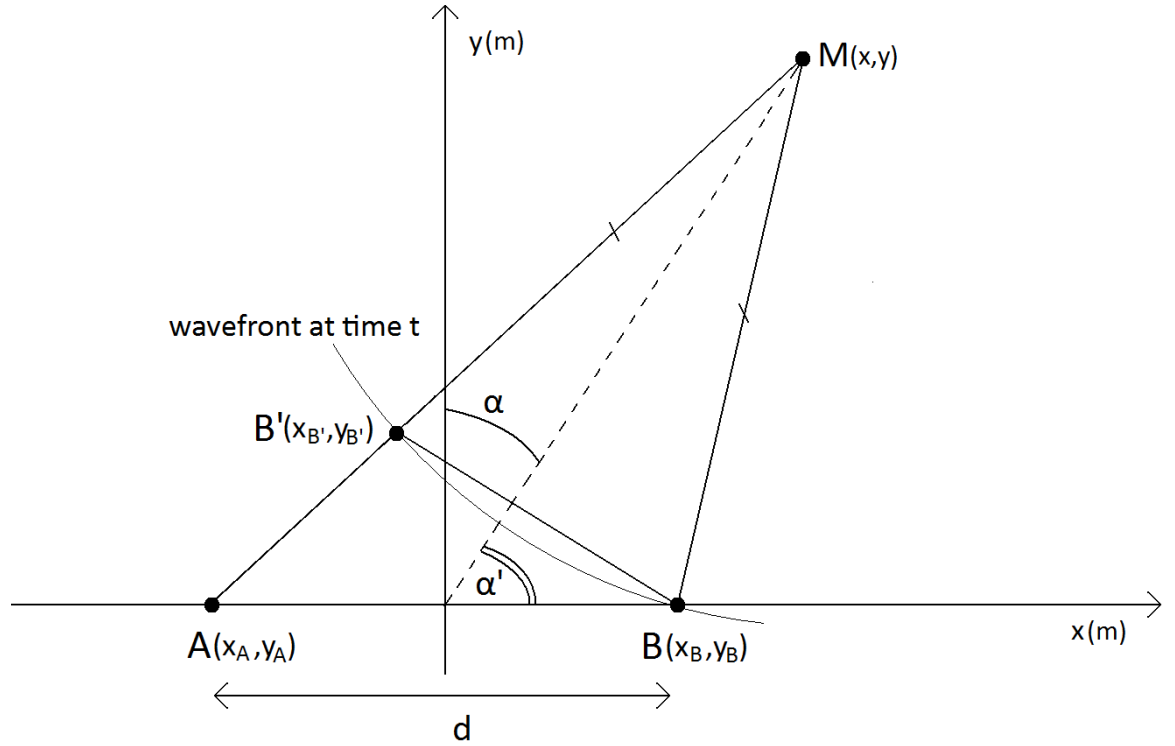
\includegraphics[width=0.7\textwidth]{../Images/sound-source-from-two-microphones.png}
    \caption{Equation formalization. Original image from \cite{Scola2010DirectionOA}}
    \label{fig:sound-source-from-two-microphones}
\end{figure}

By looking at the graphic, the following equation can be found:

\begin{equation}
    AB' = AM-B'M
\end{equation}

With Pythagorean theorem: 

\begin{equation}
    AM = \sqrt{(X_{a}-X)^2 + (Y_{a}-Y)^2}
\end{equation}
\begin{equation}
    BM = \sqrt{(X_{b}-X)^2 + (Y_{b}-Y)^2}
\end{equation}

The two microphones have the same $Y$ coordinate, so $Y_{a} = Y_{b} = Y$ and $Y_{a}-Y_{b} = 0$ and $X_{a} = -X_{B}$ The equation becomes:

\begin{equation}
    y = \pm\sqrt{\frac{AB'^2}{4} - x^2_{B} + x^2(\frac{4\cdot x^2_{B}}{AB'^2} - 1)}
\end{equation}

This setup shows that two microphones are enough to determine the direction of a sound source.
% TODO - compléter la formalisation

\section{Neural networks}

Neural networks are machine learning algorithms based on biological neurons used to solve various problems, including image recognition, speech recognition, and natural language processing. Neural networks learn from provided data to solve a problem without explicitly programming the solution. Many domains, like self-driving cars, facial recognition, and medical imaging, achieve better results using neural network models. 

A neural network (figure \ref*{fig:neural_network}) is composed of multiple neurons (the circles) that are organized in layers and connected to the neurons in the previous and next layers. 

\begin{figure}[H]
    \centering
    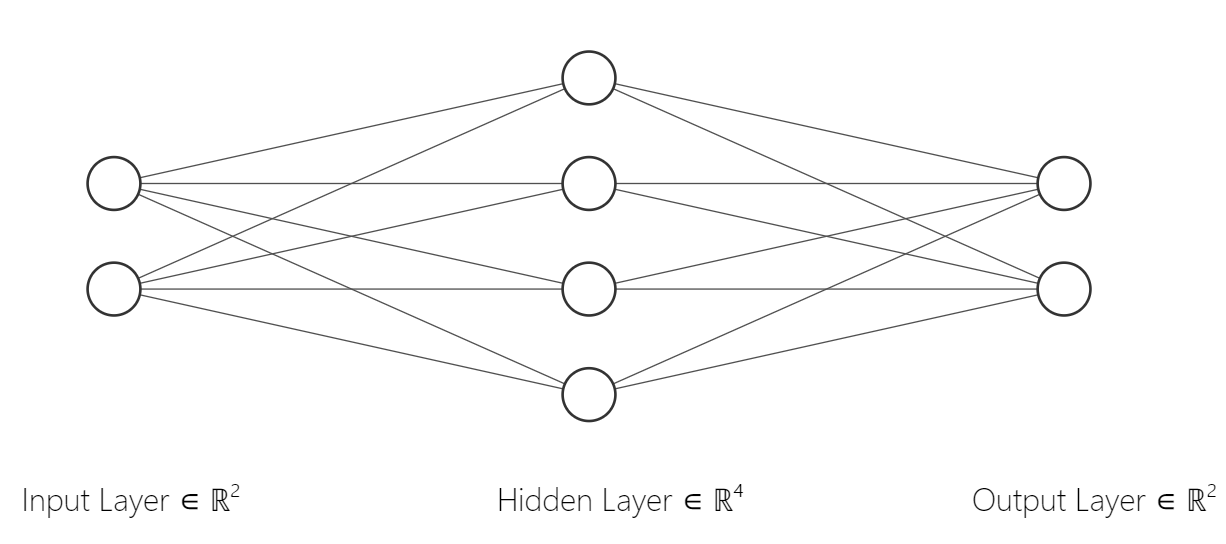
\includegraphics[width=0.7\textwidth]{../Images/neural_network_example.png}
    \caption{Neural network}
    \label{fig:neural_network}
\end{figure}

Deep neural networks are a type of neural network composed of multiple layers of neurons. They are trained on a large dataset of images and then used to classify new images. There are countless architectures \cite{LIU201711} and implementations of neural networks, but they all share the same basic principles.



\subsection{Convolutional Neural Networks}

Convolutional Neural Networks (CNNs) are neural networks used for image recognition. They use convolutional layers to extract features from images. These features are then fed into fully connected layers to perform classification. 


\subsection{Convolutional Neural Networks for source localization}

CNNs are mainly used to classify images but can also classify sounds. They are used in this thesis to classify the spectrograms of the sound signals recorded by the microphone array. The spectrograms are converted into images and fed into the CNN. The CNN then outputs a probability distribution over the possible classes. The output of the CNN gives the probability of the sound source coming from a specific direction.

\section{Related Work}

\subsection{}

